\chapter{Model development}
\label{sec:model_development}

While there could be multiple approaches to fault estimation, $REPLACE_WE$ have chosen to use a deep learning approach. The reason for this is that deep learning has shown to be very successful in many different fields, such as image classification, object detection, and image segmentation. The reason for this is that deep learning can learn the features of the data by itself, without the need for manual feature extraction. This is especially useful in $REPLACE_OUR$ case, as $REPLACE_WE$ have a large amount of data, but $REPLACE_WE$ do not know which features are important for the fault estimation.

Other possible solutions could be to use rule-based systems, which use inverse kinematics, or use frame-to-frame joint comparison to detect discreptancies, however, these are quite limited and might result in either too many false positives or false negatives. Furthermore, these rules, such as the frame-to-frame joint comparison, are not always applicable to all types of movements, and therefore might not be able to detect all types of faults in all cases.

\section{Model architecture}
\label{sec:model_architecture}

To approach the problem of error estimation, two different model architectures are devised. The first model architecture, FESDModelv1, is a deep convolutional neural network that uses the RGB, Depth, and Pose data as separate inputs. This model can be seen in figure \ref{fig:model_architecture_v1}.

\begin{figure}[htbp]
  \centering
  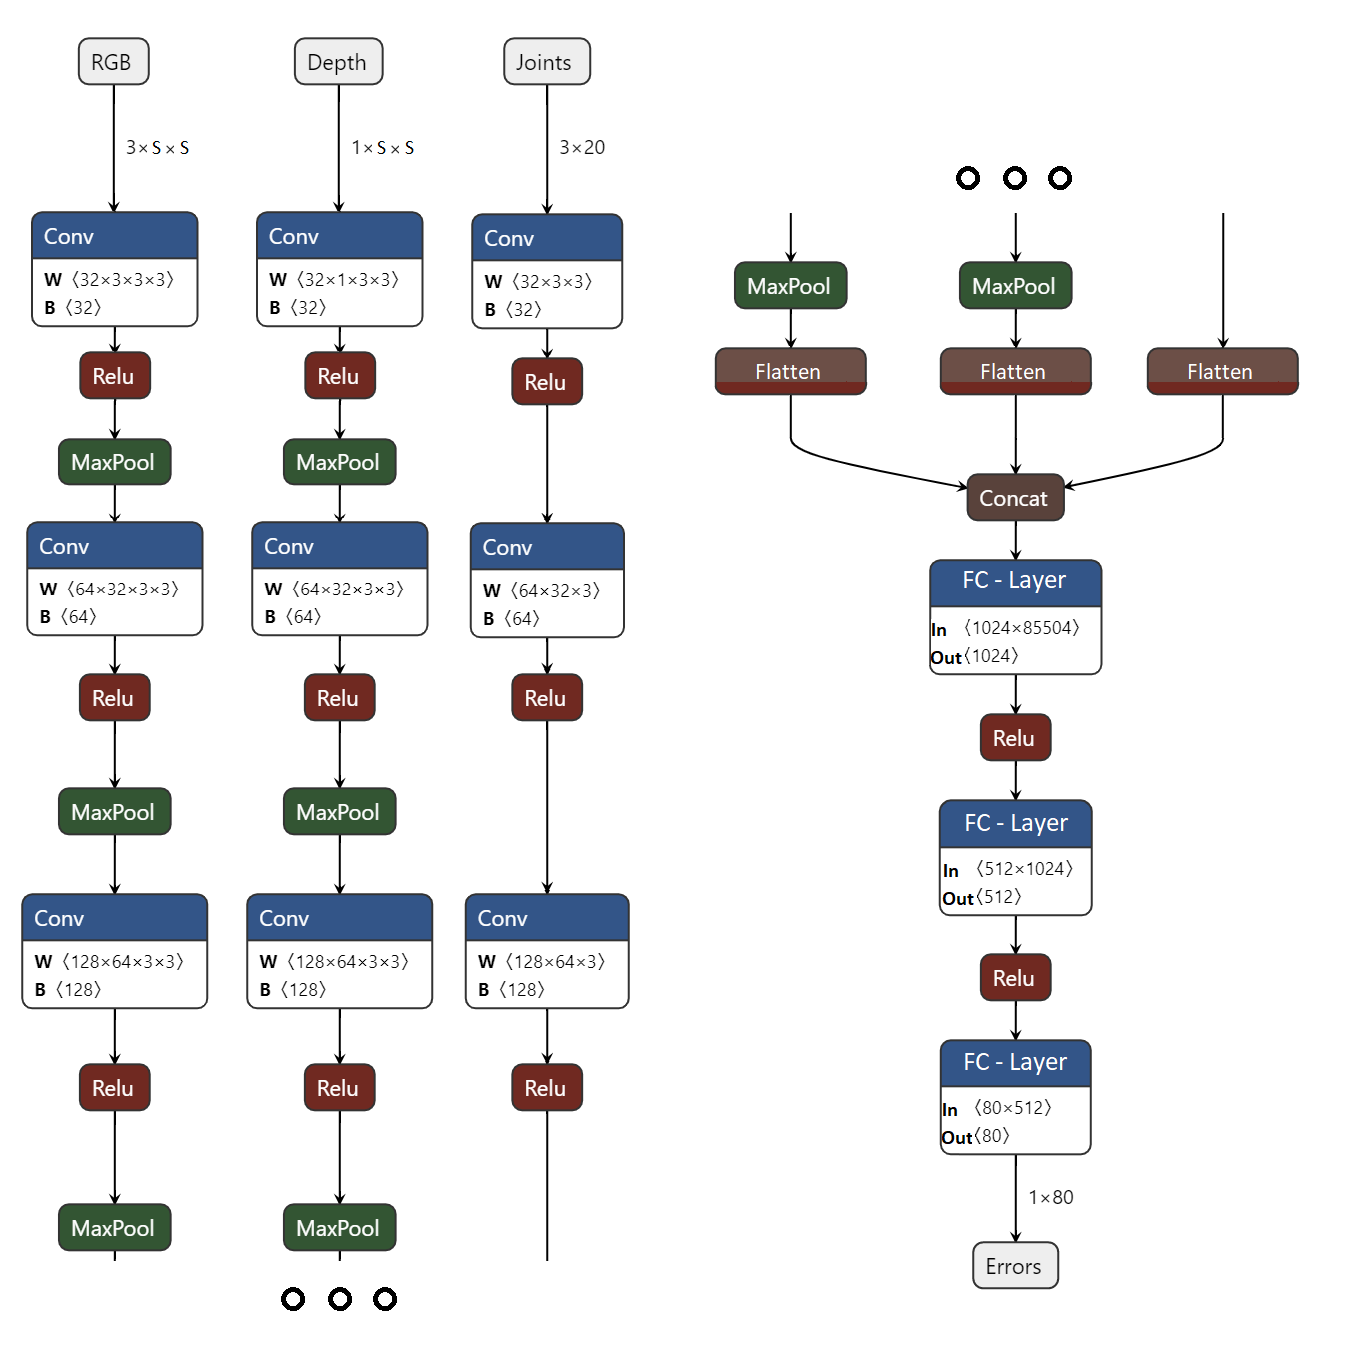
\includegraphics[width=.8\linewidth]{figures/Model/FESD.png}
  \caption[FESDModel architecture version 1]{Original FESDModel architecture with three different inputs; RGB, Depth and Joint data. With 'S' as the image size. After three convolutions the three streams are concatenated to be passed into three fully connected layers with ReLU activation functions. In this example network, the model calculates the joint problem set, therefore the output is a 1D 80 tensor of multi-object, one for each joint, i.e. 20, multi-class, one for each error class, i.e. 4, values.}
  \label{fig:model_architecture_v1}
\end{figure}

The second model architecture, FESDModelv2, utilises transfer learning to extract the features of the input data using a pre-trained model. The architecture of FESDModelv2 can be seen in figure \ref{fig:model_architecture_v2}. Both models are trained to predict the error labels for each joint. The error labels are the same as the error labels used in the data labelling explained in section \ref{sec:data_labeling}. The fully connected layers of both networks use intermittent rectified linear unit (ReLU) activation functions to combat the vanishing gradient problem by passing only the values which are greater than zero into the next layer.

\begin{figure}[htbp]
  \centering
  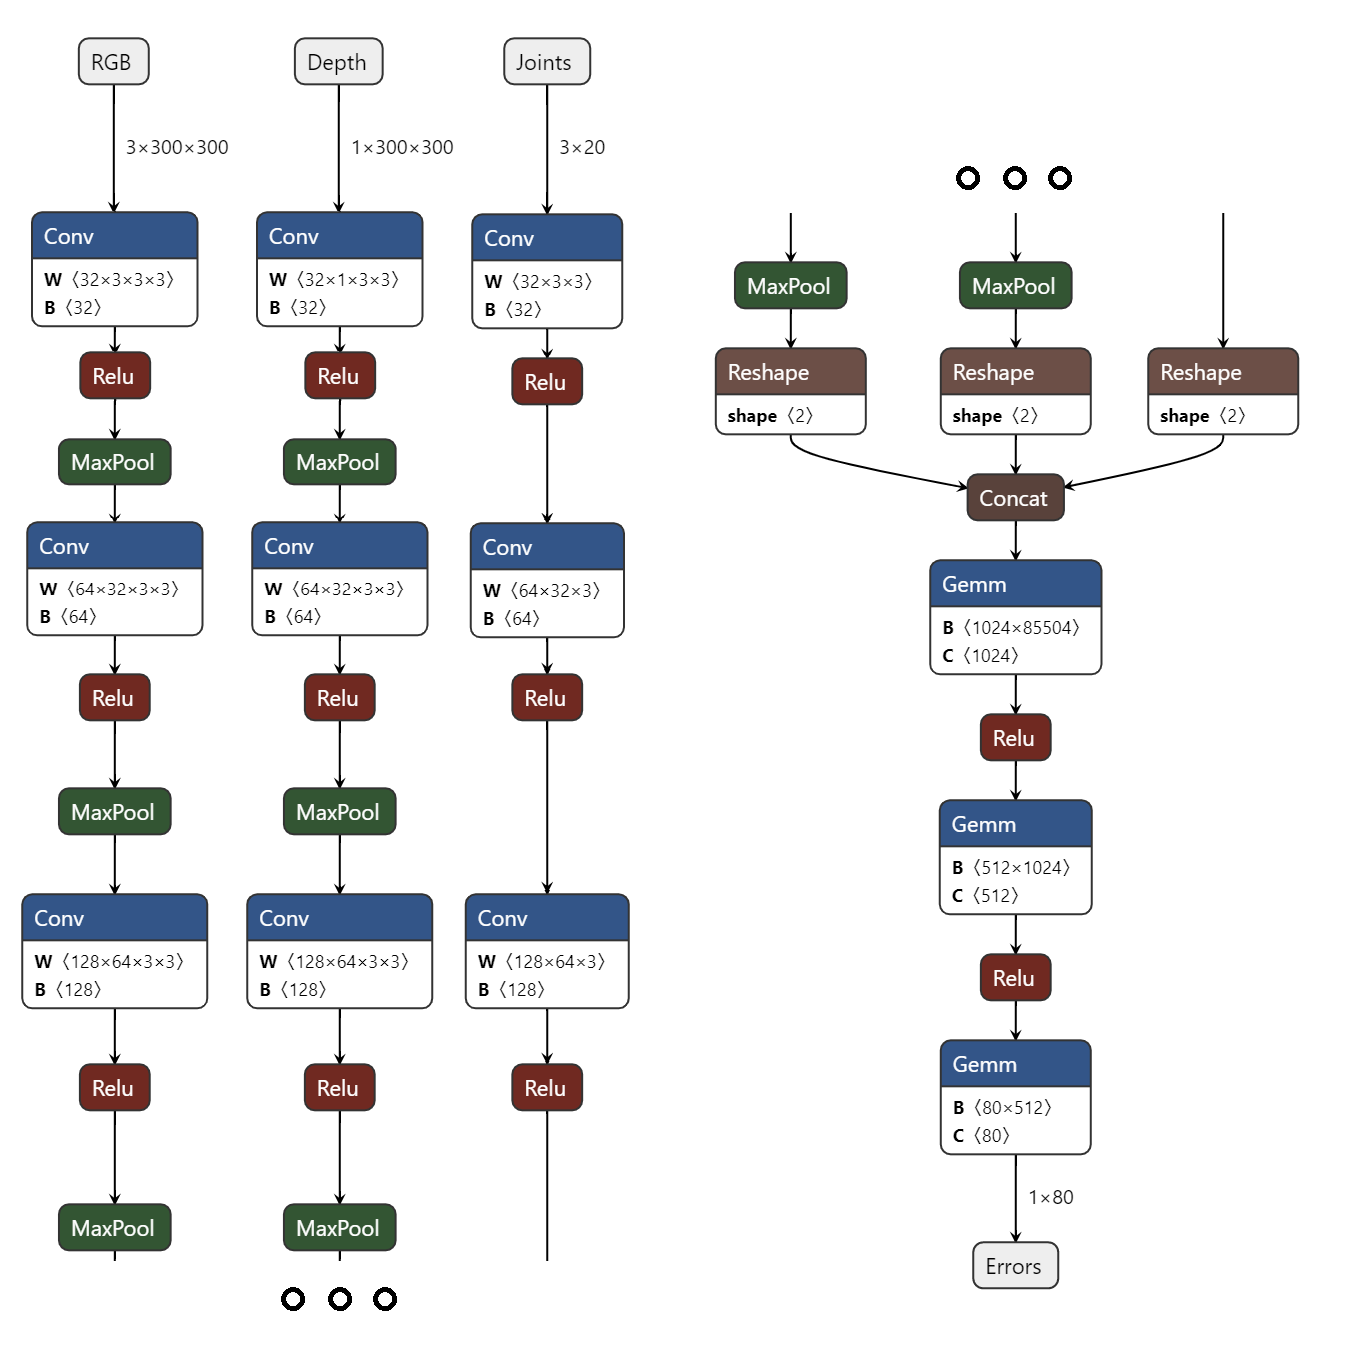
\includegraphics[width=.5\linewidth]{figures/Model/FESDv2.png}
  \caption[FESDModel architecture version 2]{FESDModelv2 architecture with transfer learning. The input is merged into a single RGB image and passed into a feature extractor. With 'S' as the image size. The feature extractor is a pre-trained EfficientNet v2 S. The output of the feature extractor is passed into two fully connected layers with ReLU activation functions. In this example network, the model calculates the joint problem set, therefore the output is a 1D 80 tensor of multi-object, one for each joint, i.e. 20, multi-class, one for each of the 4 error classes.}
  \label{fig:model_architecture_v2}
\end{figure}

While FESDModelv1 uses the data as it is stored in the dataset, FESDModelv2 merges the data into a single RGB image. This is done using the feature extractor, which is trained on RGB images. The data is merged by assigning each modality to a channel in an RGB image. The RGB image is transformed into greyscale and assigned to the red channel, the depth image is scaled to a value between 0 and 255 and assigned to the green channel, and the joint coordinates are assigned to the blue channel.

In total eight models were developed and trained. Four models were trained using FESDModelv1 and four models were trained using FESDModelv2. Each of the models corresponds to one of the problem sets introduced in section \ref{sec:problem_set}, i.e. one model for each problem set is trained using FESDModelv1 and one model for each problem set is trained using FESDModelv2.

The output of the model varies depending on the problem set. The joint problem set contains more detailed error information, which was discussed in section \ref{sec:data_labeling}. Therefore, the models developed to detect joint-level errors have an output vector of size 80, i.e. twenty joints, each with four different error labels. The other problem sets are labelled using two values to represent whether an area is faulty, "Error" or "No Error". Hence the Full Body, Half Body and Body Part problem sets have an output vector of size 2, 4, and 12 respectively.

To choose a network that is used by FESDModelv2 as a feature extractor, multiple different networks have been compared, which can be seen in figure \ref{fig:network_comparison}. One of the target applications of the model is to be used in a real-time application so that error handling can be conducted. Consequently, a lightweight model which does not impact the performance much is preferred. Therefore, the models are compared by the number of floating-point operations (FLOPS) to their Accuracy on ImageNet-1K. Table \ref{tab:network_comparison} shows the top 5 models according to their accuracy and performance. 

\begin{figure}[htbp]
  \centering
  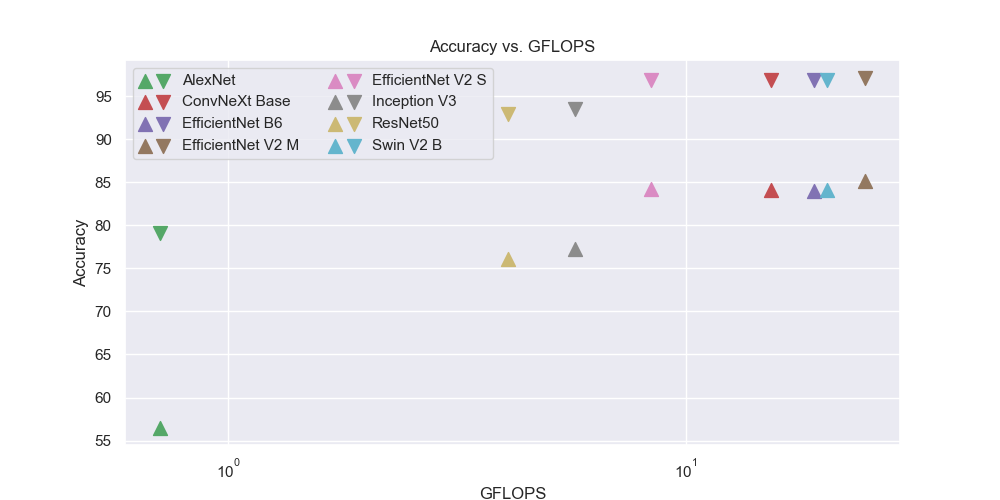
\includegraphics[width=.8\linewidth]{figures/network/networks.png}
  \caption[Network comparison]{The comparison of different networks by their GFLOPS and their Top-5 Accuracy. The models are sorted by their GFLOPS and their Top-5 Accuracy\footnote{Source: \url{https://pytorch.org/vision/main/models.html} on 08/05/2023}. The models are EfficientNet V2 S, ConvNeXt Base, EfficientNet B6, Swin V2 B, and EfficientNet V2 M. Additionally, AdamNet, ResNet-50 and Inception-v3 are added as a reference.}
  \label{fig:network_comparison}
\end{figure}

\begin{table}[htbp]
  \caption[Top 5 models for Accuracy and Performance]{The top 5 models according to their accuracy and performance. The models are sorted by their GFLOPS and their Top-5 Accuracy\footnote{Source: \url{https://pytorch.org/vision/main/models.html} on 08/05/2023}. The models are EfficientNet V2 S, ConvNeXt Base, EfficientNet B6, Swin V2 B, and EfficientNet V2 M.}
  \label{tab:network_comparison}
  \centering
  \begin{tabular}{lrrrr}
    \hline
            Weight &  Acc@1 &  Acc@5 &   Params &  GFLOPs \\
    \hline
  EfficientNet V2 S & 84.228 & 96.878 & $2.15 \times 10^7$ &   8.370 \\
      ConvNeXt Base & 84.062 & 96.870 & $8.86 \times 10^7$ &  15.360 \\
    EfficientNet B6 & 84.008 & 96.916 & $4.30 \times 10^7$ &  19.070 \\
          Swin V2 B & 84.112 & 96.864 & $8.79 \times 10^7$ &  20.320 \\
  EfficientNet V2 M & 85.112 & 97.156 & $5.41 \times 10^7$ &  24.580 \\
  \hline
  \end{tabular}
\end{table}

EfficientNet v2 was chosen since it proved to be the most performant while being the most accurate of the networks that were analysed. In particular, the small variant with $2.15 \times 10^7$ Parameters and a Top-1 Accuracy of $84.228\%$\cite{tan2021efficientnetv2}.  While EfficientNet V2 M out-performs EfficientNet V2 S in terms of Top-1 Accuracy, the number of additional parameters needed to achieve a better accuracy outway the performance bonus that EfficientNetv2 S brings with it. EfficientNetv2 is a convolutional neural network, which optimises training speed and parameter efficiency and improves upon EfficientNet\cite{tan2020efficientnet}. The main focus of EfficientNet is the scaling of the model in width, depth and resolution of the input image. 

\FloatBarrier
\section{Data preparation}
\label{sec:data_preparation}

To successfully train FESDModel three steps are taken before training can begin, data augmentation, data merging, and data balancing. The data augmentation is done to ensure that the model is robust to different variations in the data. The data merging is done to combine the different modalities into a single tensor. Since the dataset is unbalanced, the data balancing is done to ensure that the model is not biased toward any particular error label. 

The finished data preparation pipeline for FESDModelv1 and FESDModelv2 can be seen in figure \ref{fig:data_preparation_pipeline}.

\begin{figure}[ht]
  \centering
  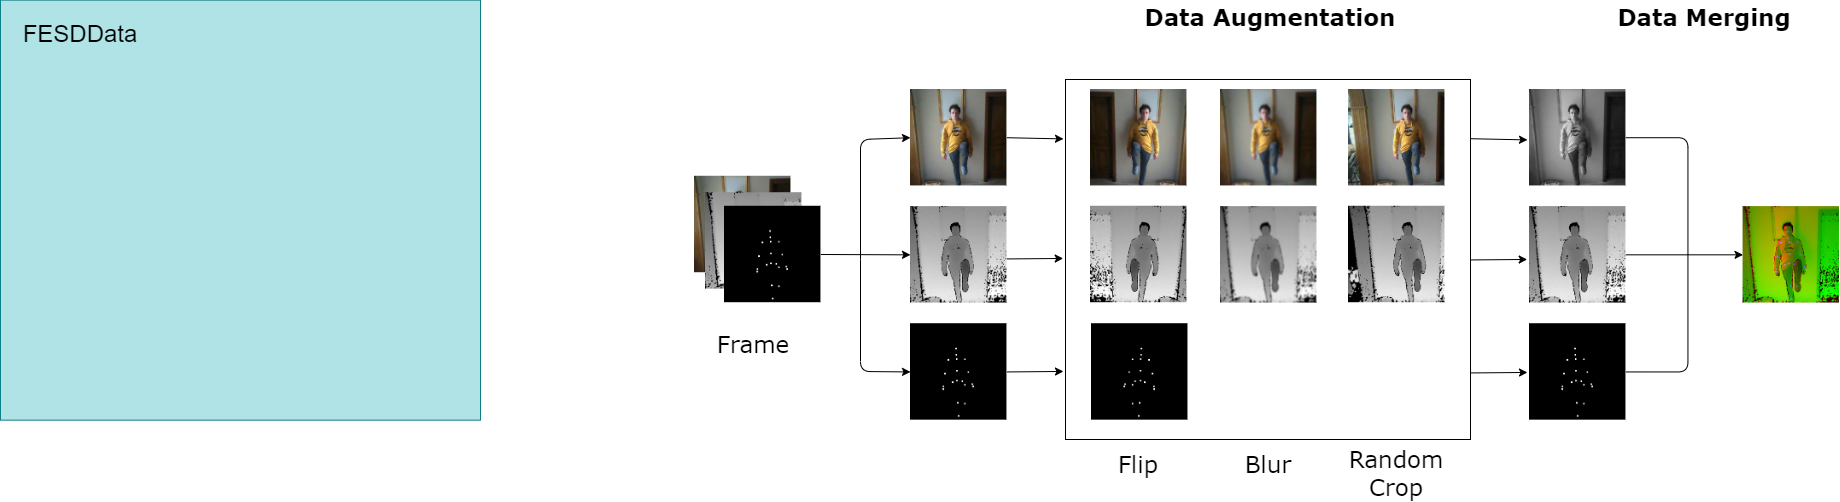
\includegraphics[width=\linewidth]{figures/ProcessingPipeline/DataProcessing.png}
  \caption[Data preparation pipeline for FESDModel]{The three modalities are separately randomly flipped, Blurred, and Cropped. For FESDModelv1 the separate modalities are passed into the network. For FESDModelv2, the RGB image is transformed into a greyscale image and all three modalities are merged into a single RGB image.}
  \label{fig:data_preparation_pipeline}
\end{figure}

The joints are stored within a JSON file containing the coordinates of each joint in 2D and 3D. To process the 2D joint data is drawn on an image that has the same dimensions as the RGB and Depth image for FESDModelv2. For FESDModelv1 the position of each joint relative to the waist joint is passed into the network.

\subsection{Data augmentation}

Four different augmentations are applied to the data to generalise the data. The first augmentation is flipping the data. The RGB image, the depth image, and the joint image are flipped horizontally. Furthermore, the ground truth data is flipped, as labels refer to the left or right side of the body, which would no longer coincide with the data that is passed into the network.

Additionally, the images are cropped at random while keeping the positions of the joints and a margin around the joints visible. This ensures that the model is robust to different positions of the user in the image. 

Finally, Gaussian noise is applied to the RGB image and the depth image. This further improves the robustness of irregular data.

The augmentations can be seen in figure \ref{fig:data_preparation_pipeline} where they are applied to a sample frame from the dataset.

\subsection{Data balancing}

In the ordinary case, HPE is not meant to produce faulty results. In the selected exercises it is aimed to produce faulty results. However, this still does not produce a balanced dataset. In section \ref{sec:dataset}, the statistics of the dataset are shown. Most notably for the problem set \textit{Half} and \textit{Full}, in figures \ref{fig:hb_pie} and \ref{fig:fb_pie}, where the error label \textit{No Error} is overrepresented it can be seen that the dataset is imbalanced.

To balance the dataset, frames are sampled using a Weighted Random Sampler for each batch of the training. The weights for the samples are calculated based on the occurrence of the error labels in the dataset. While only considering the whole body as a single object, the calculation of the weights is simple. For each frame, the error label is counted and the inverse of the count is used as the weight for the frame. This ensures that the model is not biased toward any particular error label by oversampling the frames which contain an error.

However, for the other problem sets the calculation of the weights is more complex. In the other problem sets each frame contains an error for each area, e.g. when considering the Half-Body problem, the upper and lower body 2 errors. To successfully balance the dataset for each area four weights would need to be created and balanced, i.e. the upper and lower body have an error the upper body is faulty and the lower body is not, etc. This would oversample some frames while undersampling others. In the other problem sets this is far more visible. Therefore, it was decided to consider the sum of erroneous joints per frame as a balancing factor. This means that frames that have the same number of erroneous areas are weighed the same.

\section{Model training}
\label{sec:model_training}


\section{Evaluation}
\label{sec:model_evaluation}

Finally, we evaluate our model by calculating different error metrics such as the root mean squared error as can be seen in Equation \ref{eq:rmse}, and the cross entropy loss. We also calculate the accuracy of the model, which is the percentage of correctly predicted faults. We also calculate the precision and recall of the model. The precision is the percentage of correctly predicted faults out of all predicted faults. The recall is the percentage of correctly predicted faults out of all faults in the data. We also calculate the F1 score, which is the harmonic mean of the precision and recall. The F1 score is a good indicator of the overall performance of the model.

%\begin{equation}
%Actually RMSE not a good metric for Classification, Will mention it but not in this much detail
%\label{eq:rmse}
%RMSE = \sqrt{\dfrac{1}{n}\sum_{i=0}^{n} (pred_i - gt_i)^2}
%\end{equation}

\textbf{Explain Confusion Matrix}

\textbf{Explain Cohen Kappa Metric}

\textbf{Briefly explain Accuracy, Precision, Recall and F1}

\textbf{Explain Testing}